% Options for packages loaded elsewhere
\PassOptionsToPackage{unicode}{hyperref}
\PassOptionsToPackage{hyphens}{url}
%
\documentclass[
]{article}
\usepackage{amsmath,amssymb}
\usepackage{iftex}
\ifPDFTeX
  \usepackage[T1]{fontenc}
  \usepackage[utf8]{inputenc}
  \usepackage{textcomp} % provide euro and other symbols
\else % if luatex or xetex
  \usepackage{unicode-math} % this also loads fontspec
  \defaultfontfeatures{Scale=MatchLowercase}
  \defaultfontfeatures[\rmfamily]{Ligatures=TeX,Scale=1}
\fi
\usepackage{lmodern}
\ifPDFTeX\else
  % xetex/luatex font selection
\fi
% Use upquote if available, for straight quotes in verbatim environments
\IfFileExists{upquote.sty}{\usepackage{upquote}}{}
\IfFileExists{microtype.sty}{% use microtype if available
  \usepackage[]{microtype}
  \UseMicrotypeSet[protrusion]{basicmath} % disable protrusion for tt fonts
}{}
\makeatletter
\@ifundefined{KOMAClassName}{% if non-KOMA class
  \IfFileExists{parskip.sty}{%
    \usepackage{parskip}
  }{% else
    \setlength{\parindent}{0pt}
    \setlength{\parskip}{6pt plus 2pt minus 1pt}}
}{% if KOMA class
  \KOMAoptions{parskip=half}}
\makeatother
\usepackage{xcolor}
\usepackage[margin=1in]{geometry}
\usepackage{color}
\usepackage{fancyvrb}
\newcommand{\VerbBar}{|}
\newcommand{\VERB}{\Verb[commandchars=\\\{\}]}
\DefineVerbatimEnvironment{Highlighting}{Verbatim}{commandchars=\\\{\}}
% Add ',fontsize=\small' for more characters per line
\usepackage{framed}
\definecolor{shadecolor}{RGB}{248,248,248}
\newenvironment{Shaded}{\begin{snugshade}}{\end{snugshade}}
\newcommand{\AlertTok}[1]{\textcolor[rgb]{0.94,0.16,0.16}{#1}}
\newcommand{\AnnotationTok}[1]{\textcolor[rgb]{0.56,0.35,0.01}{\textbf{\textit{#1}}}}
\newcommand{\AttributeTok}[1]{\textcolor[rgb]{0.13,0.29,0.53}{#1}}
\newcommand{\BaseNTok}[1]{\textcolor[rgb]{0.00,0.00,0.81}{#1}}
\newcommand{\BuiltInTok}[1]{#1}
\newcommand{\CharTok}[1]{\textcolor[rgb]{0.31,0.60,0.02}{#1}}
\newcommand{\CommentTok}[1]{\textcolor[rgb]{0.56,0.35,0.01}{\textit{#1}}}
\newcommand{\CommentVarTok}[1]{\textcolor[rgb]{0.56,0.35,0.01}{\textbf{\textit{#1}}}}
\newcommand{\ConstantTok}[1]{\textcolor[rgb]{0.56,0.35,0.01}{#1}}
\newcommand{\ControlFlowTok}[1]{\textcolor[rgb]{0.13,0.29,0.53}{\textbf{#1}}}
\newcommand{\DataTypeTok}[1]{\textcolor[rgb]{0.13,0.29,0.53}{#1}}
\newcommand{\DecValTok}[1]{\textcolor[rgb]{0.00,0.00,0.81}{#1}}
\newcommand{\DocumentationTok}[1]{\textcolor[rgb]{0.56,0.35,0.01}{\textbf{\textit{#1}}}}
\newcommand{\ErrorTok}[1]{\textcolor[rgb]{0.64,0.00,0.00}{\textbf{#1}}}
\newcommand{\ExtensionTok}[1]{#1}
\newcommand{\FloatTok}[1]{\textcolor[rgb]{0.00,0.00,0.81}{#1}}
\newcommand{\FunctionTok}[1]{\textcolor[rgb]{0.13,0.29,0.53}{\textbf{#1}}}
\newcommand{\ImportTok}[1]{#1}
\newcommand{\InformationTok}[1]{\textcolor[rgb]{0.56,0.35,0.01}{\textbf{\textit{#1}}}}
\newcommand{\KeywordTok}[1]{\textcolor[rgb]{0.13,0.29,0.53}{\textbf{#1}}}
\newcommand{\NormalTok}[1]{#1}
\newcommand{\OperatorTok}[1]{\textcolor[rgb]{0.81,0.36,0.00}{\textbf{#1}}}
\newcommand{\OtherTok}[1]{\textcolor[rgb]{0.56,0.35,0.01}{#1}}
\newcommand{\PreprocessorTok}[1]{\textcolor[rgb]{0.56,0.35,0.01}{\textit{#1}}}
\newcommand{\RegionMarkerTok}[1]{#1}
\newcommand{\SpecialCharTok}[1]{\textcolor[rgb]{0.81,0.36,0.00}{\textbf{#1}}}
\newcommand{\SpecialStringTok}[1]{\textcolor[rgb]{0.31,0.60,0.02}{#1}}
\newcommand{\StringTok}[1]{\textcolor[rgb]{0.31,0.60,0.02}{#1}}
\newcommand{\VariableTok}[1]{\textcolor[rgb]{0.00,0.00,0.00}{#1}}
\newcommand{\VerbatimStringTok}[1]{\textcolor[rgb]{0.31,0.60,0.02}{#1}}
\newcommand{\WarningTok}[1]{\textcolor[rgb]{0.56,0.35,0.01}{\textbf{\textit{#1}}}}
\usepackage{graphicx}
\makeatletter
\def\maxwidth{\ifdim\Gin@nat@width>\linewidth\linewidth\else\Gin@nat@width\fi}
\def\maxheight{\ifdim\Gin@nat@height>\textheight\textheight\else\Gin@nat@height\fi}
\makeatother
% Scale images if necessary, so that they will not overflow the page
% margins by default, and it is still possible to overwrite the defaults
% using explicit options in \includegraphics[width, height, ...]{}
\setkeys{Gin}{width=\maxwidth,height=\maxheight,keepaspectratio}
% Set default figure placement to htbp
\makeatletter
\def\fps@figure{htbp}
\makeatother
\setlength{\emergencystretch}{3em} % prevent overfull lines
\providecommand{\tightlist}{%
  \setlength{\itemsep}{0pt}\setlength{\parskip}{0pt}}
\setcounter{secnumdepth}{-\maxdimen} % remove section numbering
\ifLuaTeX
  \usepackage{selnolig}  % disable illegal ligatures
\fi
\IfFileExists{bookmark.sty}{\usepackage{bookmark}}{\usepackage{hyperref}}
\IfFileExists{xurl.sty}{\usepackage{xurl}}{} % add URL line breaks if available
\urlstyle{same}
\hypersetup{
  pdftitle={projet\_STA},
  pdfauthor={BOUILLON Mathis},
  hidelinks,
  pdfcreator={LaTeX via pandoc}}

\title{projet\_STA}
\author{BOUILLON Mathis}
\date{2024-12-12}

\begin{document}
\maketitle

\hypertarget{projet-de-suxe9ries-temporelles-avancuxe9es}{%
\section{Projet de Séries Temporelles
Avancées}\label{projet-de-suxe9ries-temporelles-avancuxe9es}}

\hypertarget{moduxe8le-ardl-une-duxe9finition-formelle}{%
\subsubsection{Modèle ARDL : une définition
formelle}\label{moduxe8le-ardl-une-duxe9finition-formelle}}

Le modèle ARDL (AutoRegressive Distributed Lag) est une spécification
économétrique qui permet de modéliser la relation dynamique entre une
variable dépendante \(y_t\) et un ensemble de variables explicatives
\(x_{it}\).

La forme générale d'un modèle ARDL(p, q) peut s'écrire comme suit :

\[
y_t = \alpha + \sum_{i=1}^p \phi_i y_{t-i} + \sum_{j=0}^q \sum_{i=1}^k \beta_{ij} x_{i,t-j} + \varepsilon_t
\]

où :

\begin{itemize}
\tightlist
\item
  \(y_t\) est la variable dépendante à l'instant \(t\),
\item
  \(x_{i,t-j}\) sont les variables explicatives (avec \(i = 1, ..., k\)
  et \(j = 0, ..., q\) pour capturer les décalages),
\item
  \(\alpha\) est la constante,
\item
  \(\phi_i\) sont les coefficients des termes autorégressifs,
\item
  \(\beta_{ij}\) sont les coefficients des termes à retards distribués,
\item
  \(\varepsilon_t\) est le terme d'erreur.
\end{itemize}

Ce modèle est utilisé pour analyser les relations à court terme et à
long terme entre les variables. En cas de cointégration entre \(y_t\) et
\(x_{it}\), une transformation du modèle ARDL en un modèle de correction
d'erreur (ECM) permet de quantifier les ajustements vers l'équilibre de
long terme.

p est l'ordre de l'AR, et q est le nombre de retards appliqué aux
variables explicatives ou exogènes au modèle.

\hypertarget{ruxe9cupuxe9ration-des-donnuxe9es-du-cac-40-et-visualisation}{%
\section{Récupération des données du CAC 40 et visualisation
:}\label{ruxe9cupuxe9ration-des-donnuxe9es-du-cac-40-et-visualisation}}

\begin{Shaded}
\begin{Highlighting}[]
\CommentTok{\# Télécharger les données du CAC 40}
\NormalTok{cac40 }\OtherTok{\textless{}{-}} \FunctionTok{getSymbols}\NormalTok{(}\StringTok{"\^{}FCHI"}\NormalTok{, }\AttributeTok{src =} \StringTok{"yahoo"}\NormalTok{, }\AttributeTok{from =} \StringTok{"1990{-}01{-}01"}\NormalTok{, }\AttributeTok{to =} \StringTok{"2023{-}12{-}31"}\NormalTok{, }\AttributeTok{auto.assign =} \ConstantTok{FALSE}\NormalTok{)}
\end{Highlighting}
\end{Shaded}

\begin{verbatim}
## Warning: ^FCHI contains missing values. Some functions will not work if objects
## contain missing values in the middle of the series. Consider using na.omit(),
## na.approx(), na.fill(), etc to remove or replace them.
\end{verbatim}

\begin{Shaded}
\begin{Highlighting}[]
\CommentTok{\# Extraire uniquement les prix de clôture}
\NormalTok{cac40\_close }\OtherTok{\textless{}{-}} \FunctionTok{na.omit}\NormalTok{(}\FunctionTok{Cl}\NormalTok{(cac40))  }\CommentTok{\# \textquotesingle{}Cl()\textquotesingle{} extrait la colonne de clôture}
\CommentTok{\#nous pouvons également considérer d\textquotesingle{}autres indicateurs tq le max sur la journée, le min...}
\FunctionTok{colnames}\NormalTok{(cac40\_close) }\OtherTok{\textless{}{-}} \StringTok{"Close"}

\CommentTok{\#Visualisation de la série }

\FunctionTok{autoplot}\NormalTok{(cac40\_close) }\SpecialCharTok{+}
  \FunctionTok{ggtitle}\NormalTok{(}\StringTok{"Indice CAC 40 pour la période 1990{-}2023"}\NormalTok{) }\SpecialCharTok{+}
  \FunctionTok{xlab}\NormalTok{(}\StringTok{"Date"}\NormalTok{) }\SpecialCharTok{+}
  \FunctionTok{ylab}\NormalTok{(}\StringTok{"Clôture"}\NormalTok{) }\SpecialCharTok{+}
  \FunctionTok{theme\_minimal}\NormalTok{() }\SpecialCharTok{+} 
  \FunctionTok{theme}\NormalTok{(}\AttributeTok{plot.title =} \FunctionTok{element\_text}\NormalTok{(}\AttributeTok{hjust =} \FloatTok{0.5}\NormalTok{)) }
\end{Highlighting}
\end{Shaded}

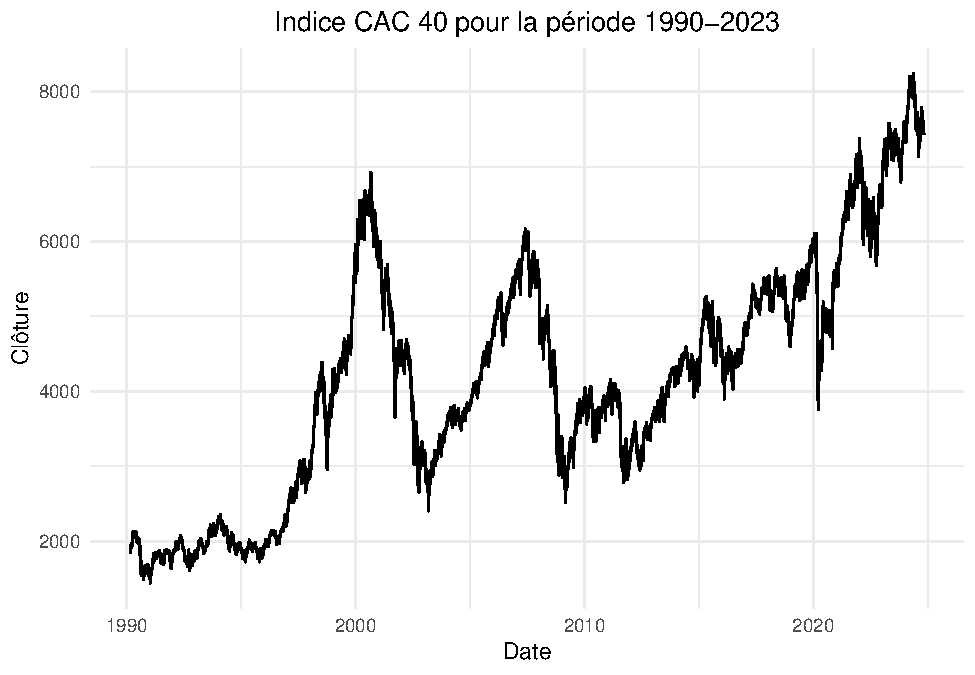
\includegraphics{projet_STA_files/figure-latex/unnamed-chunk-2-1.pdf}

Nous pouvons déjà voir que la série présente une tendance linéaire
claire. Il n'y a pas forcément de saisonnalité (plutôt des grosses
chutes lors des crises globales)

\hypertarget{analyse-pruxe9liminaire-de-la-suxe9rie-de-lindice}{%
\section{Analyse préliminaire de la série de
l'indice}\label{analyse-pruxe9liminaire-de-la-suxe9rie-de-lindice}}

\hypertarget{valeurs-manquantes}{%
\subsection{Valeurs manquantes}\label{valeurs-manquantes}}

\begin{Shaded}
\begin{Highlighting}[]
\CommentTok{\# Vérifier s\textquotesingle{}il y a des valeurs manquantes dans la série}
\NormalTok{missing\_values }\OtherTok{\textless{}{-}} \FunctionTok{sum}\NormalTok{(}\FunctionTok{is.na}\NormalTok{(cac40\_close))}

\CommentTok{\# Afficher le nombre de valeurs manquantes}
\FunctionTok{print}\NormalTok{(}\FunctionTok{paste}\NormalTok{(}\StringTok{"Nombre de valeurs manquantes :"}\NormalTok{, missing\_values))}
\end{Highlighting}
\end{Shaded}

\begin{verbatim}
## [1] "Nombre de valeurs manquantes : 0"
\end{verbatim}

\begin{Shaded}
\begin{Highlighting}[]
\CommentTok{\# Si des valeurs manquantes existent, afficher leurs dates}
\ControlFlowTok{if}\NormalTok{ (missing\_values }\SpecialCharTok{\textgreater{}} \DecValTok{0}\NormalTok{) \{}
\NormalTok{  missing\_dates }\OtherTok{\textless{}{-}} \FunctionTok{index}\NormalTok{(cac40\_close)[}\FunctionTok{is.na}\NormalTok{(cac40\_close)]}
  \FunctionTok{print}\NormalTok{(}\StringTok{"Dates avec valeurs manquantes :"}\NormalTok{)}
  \FunctionTok{print}\NormalTok{(missing\_dates)}
\NormalTok{\} }\ControlFlowTok{else}\NormalTok{ \{}
  \FunctionTok{print}\NormalTok{(}\StringTok{"Aucune valeur manquante dans la série."}\NormalTok{)}
\NormalTok{\}}
\end{Highlighting}
\end{Shaded}

\begin{verbatim}
## [1] "Aucune valeur manquante dans la série."
\end{verbatim}

La série ne présente pas de valeurs manquantes.

\hypertarget{stat-desc}{%
\subsection{Stat desc}\label{stat-desc}}

\begin{Shaded}
\begin{Highlighting}[]
\FunctionTok{basicStats}\NormalTok{(cac40\_close)}
\end{Highlighting}
\end{Shaded}

\begin{verbatim}
##                     Close
## nobs         8.590000e+03
## NAs          0.000000e+00
## Minimum      1.441000e+03
## Maximum      7.596910e+03
## 1. Quartile  3.002600e+03
## 3. Quartile  5.189972e+03
## Mean         4.094829e+03
## Median       4.122800e+03
## Sum          3.517458e+07
## SE Mean      1.621398e+01
## LCL Mean     4.063046e+03
## UCL Mean     4.126612e+03
## Variance     2.258251e+06
## Stdev        1.502748e+03
## Skewness     9.921800e-02
## Kurtosis    -7.846610e-01
\end{verbatim}

\hypertarget{observation-de-la-tendance-linuxe9aire}{%
\subsection{Observation de la tendance
(linéaire)}\label{observation-de-la-tendance-linuxe9aire}}

\begin{Shaded}
\begin{Highlighting}[]
\CommentTok{\#graphiquement }

\CommentTok{\# Ajouter une tendance linéaire}
\FunctionTok{autoplot}\NormalTok{(cac40\_close) }\SpecialCharTok{+}
  \FunctionTok{geom\_smooth}\NormalTok{(}\AttributeTok{method =} \StringTok{"lm"}\NormalTok{, }\AttributeTok{se =} \ConstantTok{FALSE}\NormalTok{, }\AttributeTok{color =} \StringTok{"red"}\NormalTok{) }\SpecialCharTok{+}
  \FunctionTok{ggtitle}\NormalTok{(}\StringTok{"Tendance linéaire de l\textquotesingle{}indice CAC 40"}\NormalTok{) }\SpecialCharTok{+}
  \FunctionTok{xlab}\NormalTok{(}\StringTok{"Date"}\NormalTok{) }\SpecialCharTok{+}
  \FunctionTok{ylab}\NormalTok{(}\StringTok{"Clôture"}\NormalTok{) }\SpecialCharTok{+}
  \FunctionTok{theme\_minimal}\NormalTok{()}
\end{Highlighting}
\end{Shaded}

\begin{verbatim}
## `geom_smooth()` using formula = 'y ~ x'
\end{verbatim}

\includegraphics{projet_STA_files/figure-latex/unnamed-chunk-5-1.pdf}

\begin{Shaded}
\begin{Highlighting}[]
\CommentTok{\#avec le R**2}

\CommentTok{\# Créer une variable temporelle}
\NormalTok{time }\OtherTok{\textless{}{-}} \FunctionTok{as.numeric}\NormalTok{(}\FunctionTok{index}\NormalTok{(cac40\_close))}

\CommentTok{\# Ajuster un modèle linéaire : Prix \textasciitilde{} Temps}
\NormalTok{lm\_model }\OtherTok{\textless{}{-}} \FunctionTok{lm}\NormalTok{(}\FunctionTok{coredata}\NormalTok{(cac40\_close) }\SpecialCharTok{\textasciitilde{}}\NormalTok{ time)}

\CommentTok{\# Résumé du modèle}
\FunctionTok{summary}\NormalTok{(lm\_model)}
\end{Highlighting}
\end{Shaded}

\begin{verbatim}
## 
## Call:
## lm(formula = coredata(cac40_close) ~ time)
## 
## Residuals:
##     Min      1Q  Median      3Q     Max 
## -1863.6  -683.0  -277.1   606.1  3586.8 
## 
## Coefficients:
##               Estimate Std. Error t value Pr(>|t|)    
## (Intercept) -249.16433   41.68769  -5.977 2.36e-09 ***
## time           0.31995    0.00297 107.727  < 2e-16 ***
## ---
## Signif. codes:  0 '***' 0.001 '**' 0.01 '*' 0.05 '.' 0.1 ' ' 1
## 
## Residual standard error: 980.1 on 8588 degrees of freedom
## Multiple R-squared:  0.5747, Adjusted R-squared:  0.5747 
## F-statistic: 1.161e+04 on 1 and 8588 DF,  p-value: < 2.2e-16
\end{verbatim}

\hypertarget{duxe9tection-de-la-saisonnalituxe9}{%
\subsection{détection de la
saisonnalité}\label{duxe9tection-de-la-saisonnalituxe9}}

\begin{Shaded}
\begin{Highlighting}[]
\CommentTok{\# Convertir la série en périodicité mensuelle}
\NormalTok{cac40\_monthly }\OtherTok{\textless{}{-}} \FunctionTok{to.monthly}\NormalTok{(cac40\_close, }\AttributeTok{indexAt =} \StringTok{"lastof"}\NormalTok{, }\AttributeTok{OHLC =} \ConstantTok{FALSE}\NormalTok{)}

\CommentTok{\# Visualisation des moyennes mensuelles}
\NormalTok{cac40\_monthly\_mean }\OtherTok{\textless{}{-}} \FunctionTok{aggregate}\NormalTok{(cac40\_monthly, as.yearmon, mean)}

\FunctionTok{autoplot}\NormalTok{(cac40\_monthly\_mean) }\SpecialCharTok{+}
  \FunctionTok{ggtitle}\NormalTok{(}\StringTok{"Moyennes mensuelles de l\textquotesingle{}indice CAC 40"}\NormalTok{) }\SpecialCharTok{+}
  \FunctionTok{xlab}\NormalTok{(}\StringTok{"Date"}\NormalTok{) }\SpecialCharTok{+}
  \FunctionTok{ylab}\NormalTok{(}\StringTok{"Moyenne mensuelle de clôture"}\NormalTok{) }\SpecialCharTok{+}
  \FunctionTok{theme\_minimal}\NormalTok{()}
\end{Highlighting}
\end{Shaded}

\includegraphics{projet_STA_files/figure-latex/unnamed-chunk-7-1.pdf}

\hypertarget{duxe9tection-des-outliers}{%
\subsection{détection des outliers}\label{duxe9tection-des-outliers}}

\begin{Shaded}
\begin{Highlighting}[]
\CommentTok{\# Détection visuelle avec boxplot}
\FunctionTok{boxplot}\NormalTok{(}\FunctionTok{coredata}\NormalTok{(cac40\_close), }\AttributeTok{main =} \StringTok{"Détection des outliers"}\NormalTok{,}
        \AttributeTok{ylab =} \StringTok{"Prix de clôture"}\NormalTok{, }\AttributeTok{col =} \StringTok{"lightblue"}\NormalTok{)}
\end{Highlighting}
\end{Shaded}

\includegraphics{projet_STA_files/figure-latex/unnamed-chunk-8-1.pdf}

\begin{Shaded}
\begin{Highlighting}[]
\CommentTok{\# Repérer les outliers par quantile}
\NormalTok{q1 }\OtherTok{\textless{}{-}} \FunctionTok{quantile}\NormalTok{(cac40\_close, }\FloatTok{0.25}\NormalTok{)}
\NormalTok{q3 }\OtherTok{\textless{}{-}} \FunctionTok{quantile}\NormalTok{(cac40\_close, }\FloatTok{0.75}\NormalTok{)}
\NormalTok{iqr }\OtherTok{\textless{}{-}}\NormalTok{ q3 }\SpecialCharTok{{-}}\NormalTok{ q1}
\NormalTok{outliers }\OtherTok{\textless{}{-}}\NormalTok{ cac40\_close[cac40\_close }\SpecialCharTok{\textless{}}\NormalTok{ (q1 }\SpecialCharTok{{-}} \FloatTok{1.5} \SpecialCharTok{*}\NormalTok{ iqr) }\SpecialCharTok{|}\NormalTok{ cac40\_close }\SpecialCharTok{\textgreater{}}\NormalTok{ (q3 }\SpecialCharTok{+} \FloatTok{1.5} \SpecialCharTok{*}\NormalTok{ iqr)]}

\FunctionTok{print}\NormalTok{(}\StringTok{"Outliers détectés :"}\NormalTok{)}
\end{Highlighting}
\end{Shaded}

\begin{verbatim}
## [1] "Outliers détectés :"
\end{verbatim}

\begin{Shaded}
\begin{Highlighting}[]
\FunctionTok{print}\NormalTok{(outliers)}
\end{Highlighting}
\end{Shaded}

\begin{verbatim}
##      Close
\end{verbatim}

Nous allons maintenant regarder les log returns de cette série (ce qui
est équivalent à une première différenciation de la série) afin de voir
si elle est stationnaire ou non

\begin{Shaded}
\begin{Highlighting}[]
\CommentTok{\# Calcul des rendements logarithmiques}
\NormalTok{log\_returns }\OtherTok{\textless{}{-}} \FunctionTok{diff}\NormalTok{(}\FunctionTok{log}\NormalTok{(cac40\_close))}

\CommentTok{\# Visualisation des rendements}
\FunctionTok{autoplot}\NormalTok{(log\_returns) }\SpecialCharTok{+}
  \FunctionTok{ggtitle}\NormalTok{(}\StringTok{"Rendements logarithmiques du CAC 40"}\NormalTok{) }\SpecialCharTok{+}
  \FunctionTok{xlab}\NormalTok{(}\StringTok{"Date"}\NormalTok{) }\SpecialCharTok{+}
  \FunctionTok{ylab}\NormalTok{(}\StringTok{"Log{-}returns"}\NormalTok{) }\SpecialCharTok{+}
  \FunctionTok{theme\_minimal}\NormalTok{()}
\end{Highlighting}
\end{Shaded}

\begin{verbatim}
## Warning: Removed 1 row containing missing values (`geom_line()`).
\end{verbatim}

\includegraphics{projet_STA_files/figure-latex/unnamed-chunk-9-1.pdf}

\begin{Shaded}
\begin{Highlighting}[]
\CommentTok{\# Statistiques descriptives des rendements}
\FunctionTok{basicStats}\NormalTok{(log\_returns)}
\end{Highlighting}
\end{Shaded}

\begin{verbatim}
##                   Close
## nobs        8590.000000
## NAs            1.000000
## Minimum       -0.130983
## Maximum        0.105946
## 1. Quartile   -0.006494
## 3. Quartile    0.007279
## Mean           0.000165
## Median         0.000440
## Sum            1.415236
## SE Mean        0.000146
## LCL Mean      -0.000122
## UCL Mean       0.000452
## Variance       0.000184
## Stdev          0.013570
## Skewness      -0.195928
## Kurtosis       5.798655
\end{verbatim}

\begin{Shaded}
\begin{Highlighting}[]
\CommentTok{\# Histogramme des rendements}
\FunctionTok{ggplot}\NormalTok{(}\AttributeTok{data =} \FunctionTok{data.frame}\NormalTok{(}\AttributeTok{log\_returns =} \FunctionTok{coredata}\NormalTok{(log\_returns)), }\FunctionTok{aes}\NormalTok{(}\AttributeTok{x =}\NormalTok{ log\_returns)) }\SpecialCharTok{+}
  \FunctionTok{geom\_histogram}\NormalTok{(}\AttributeTok{bins =} \DecValTok{50}\NormalTok{, }\AttributeTok{fill =} \StringTok{"lightblue"}\NormalTok{, }\AttributeTok{color =} \StringTok{"black"}\NormalTok{) }\SpecialCharTok{+}
  \FunctionTok{ggtitle}\NormalTok{(}\StringTok{"Distribution des rendements logarithmiques"}\NormalTok{) }\SpecialCharTok{+}
  \FunctionTok{xlab}\NormalTok{(}\StringTok{"Log{-}returns"}\NormalTok{) }\SpecialCharTok{+}
  \FunctionTok{ylab}\NormalTok{(}\StringTok{"Fréquence"}\NormalTok{) }\SpecialCharTok{+}
  \FunctionTok{theme\_minimal}\NormalTok{()}
\end{Highlighting}
\end{Shaded}

\begin{verbatim}
## Don't know how to automatically pick scale for object of type <xts/zoo>.
## Defaulting to continuous.
\end{verbatim}

\begin{verbatim}
## Warning: Removed 1 rows containing non-finite values (`stat_bin()`).
\end{verbatim}

\includegraphics{projet_STA_files/figure-latex/unnamed-chunk-9-2.pdf}

On checke la stationnarité de la série avec un test de Dickey :

\begin{Shaded}
\begin{Highlighting}[]
\CommentTok{\# Calcul des log{-}returns}
\NormalTok{log\_returns }\OtherTok{\textless{}{-}} \FunctionTok{diff}\NormalTok{(}\FunctionTok{log}\NormalTok{(cac40\_close))}

\CommentTok{\# Test ADF sur les rendements logarithmiques}
\NormalTok{adf\_test }\OtherTok{\textless{}{-}} \FunctionTok{adf.test}\NormalTok{(}\FunctionTok{na.omit}\NormalTok{(log\_returns))}
\end{Highlighting}
\end{Shaded}

\begin{verbatim}
## Warning in adf.test(na.omit(log_returns)): p-value smaller than printed p-value
\end{verbatim}

\begin{Shaded}
\begin{Highlighting}[]
\CommentTok{\# Afficher les résultats du test}
\FunctionTok{print}\NormalTok{(adf\_test)}
\end{Highlighting}
\end{Shaded}

\begin{verbatim}
## 
##  Augmented Dickey-Fuller Test
## 
## data:  na.omit(log_returns)
## Dickey-Fuller = -20.783, Lag order = 20, p-value = 0.01
## alternative hypothesis: stationary
\end{verbatim}

La série des rendements est bien stationnaire. Nous pouvons également le
tester avec le test KPSS :

\begin{Shaded}
\begin{Highlighting}[]
\CommentTok{\# Calcul des log{-}returns}
\NormalTok{log\_returns }\OtherTok{\textless{}{-}} \FunctionTok{diff}\NormalTok{(}\FunctionTok{log}\NormalTok{(cac40\_close))}

\CommentTok{\# Test KPSS sur les rendements logarithmiques}
\NormalTok{kpss\_test }\OtherTok{\textless{}{-}} \FunctionTok{ur.kpss}\NormalTok{(}\FunctionTok{na.omit}\NormalTok{(log\_returns))}

\CommentTok{\# Résumé des résultats}
\FunctionTok{summary}\NormalTok{(kpss\_test)}
\end{Highlighting}
\end{Shaded}

\begin{verbatim}
## 
## ####################### 
## # KPSS Unit Root Test # 
## ####################### 
## 
## Test is of type: mu with 12 lags. 
## 
## Value of test-statistic is: 0.0543 
## 
## Critical value for a significance level of: 
##                 10pct  5pct 2.5pct  1pct
## critical values 0.347 0.463  0.574 0.739
\end{verbatim}

Le test-statistic obtenu (0.0543) est bien inférieur à toutes les
valeurs critiques obtenues à pour chaque seuil. Cela signifie que nous
ne rejetons pas l'hypothèse nulle i.e.~que les rendements logarithmiques
du CAC 40 sont stationnaires autour d'une moyenne constante.

\end{document}
